\section{Lineare Programmierung \skript{49}}

\subsection{Problemformulierung}
  \subsubsection{Notationen}
    \begin{tabular}{p{6cm} l}
      Variablen (Spalten) & $x \in \mathbb{R}^n$; $I = \{1, ..., m\}$ \\
      Constraints ((Un-)gleichungen; Zeilen) & $a^k$; $J = \{1, ..., m\}$ \\
      Matrix & $A \in \mathbb{R}^{m \times n}$
    \end{tabular}
    
    \begin{tabularx}{\textwidth}{|X|p{4.5cm}|p{5.5cm}|p{2cm}|}
    \hline
      Lineares Problem (Beispiel U4-1)
        & $\max x_1 + 3 x_2 + 2x_3$
        & $x_2 + x_3 \leq 2$ \newline 
          $x_1 - 2x_2 \leq -2$
        & $x_1, x_2, x_3 \geq 0$\\
      \hline
      \hline
      Zeilennotation
        & $\max c x$ \newline
        $c$ = Zeilenvektor $1 \times n$\newline
        $x$ = Spaltenvektor $n \times 1$
        & $a^i x \leq b_i, \;i=1,...,m$ \newline
        $a^i$ = Zeilenvektor $1 \times n$\newline
        $x$ = Spaltenvektor $n \times 1$
        & $x \geq 0$\\
      Beispiel
        & $\max [1, 3, 2]
          \begin{bmatrix}
            x_1\\x_2\\x_3
          \end{bmatrix}$
        & $a^1: \; [0,1,1]
          \begin{bmatrix}
            x_1\\x_2\\x_3
          \end{bmatrix} \leq 2$\newline
          $a^2: \; [1,-2,0]
          \begin{bmatrix}
            x_1\\x_2\\x_3
          \end{bmatrix} \leq -2$
        & $x \geq 0$
        \\
      \hline
      Spaltennotation
        & $\max c x$ \newline
        $c$ = Zeilenvektor $1 \times n$\newline
        $x$ = Spaltenvektor $n \times 1$
        & $\sum\limits_{j=1}^{n}A_j x_j \leq b$ \newline
        $A_j$ = Spaltenvektor $n \times 1$ \newline 
        $b$ = Spaltenvektor $n \times 1$
        & $x \geq 0$
        \\
      Beispiel
        & $\max [1,3,2]
          \begin{bmatrix}
            x_1\\x_2\\x_3
          \end{bmatrix}$
        & $\begin{bmatrix}
            0\\1
          \end{bmatrix} x_1 + 
          \begin{bmatrix}
            1\\-2
          \end{bmatrix} x_2 + 
          \begin{bmatrix}
            1\\0
          \end{bmatrix} x_3
          \leq \begin{bmatrix}
            2 \\ -2
          \end{bmatrix}$
        &  $x \geq 0$
        \\
      \hline
      Matrixnotation
        & $\max c x$ \newline
        $c$ = Zeilenvektor $1 \times n$\newline
        $x$ = Spaltenvektor $n \times 1$
        & $A x \leq b$ \newline
        $A$ = Matrix $m \times n$\newline
        $b$ = Spaltenvektor $m \times 1$
        & $x \geq 0$
        \\
      Beispiel
        & $\max [1, 3, 2]
          \begin{bmatrix}
            x_1\\x_2\\x_3
          \end{bmatrix}$
        & $\begin{bmatrix}
            0& 1 & 1\\
            1& -2 & 0
          \end{bmatrix}
          \begin{bmatrix}
            x_1\\x_2\\x_3
          \end{bmatrix}
          \leq \begin{bmatrix}
            2 \\ -2
          \end{bmatrix}$
        &  $x \geq 0$
        \\
      \hline
    \end{tabularx}


  \subsubsection{Normalformen}
    Ein lineares Programm kann in verschiedenen Formen geschrieben werden:
    
    \begin{tabularx}{\textwidth}{|l|X|}
      \hline
      Allgemeine Form & 
          max / min $cx$ \newline
          $a^ix \leq b_i,$ \newline
          $a^ix = b_i,$ \newline
          $a^ix \geq b_i,$ \newline
          $x_j \geq 0,$ \newline
          $x_j \text{ frei},$ \newline
          $x_j \leq 0$
          \\
      \hline
      Kanonische Form & 
          max $cx$ \newline
          $a^ix \leq b_i,$ \newline
          $x_j \geq 0$ \newline
          \em oder \em\newline
          min $cx$ \newline
          $a^ix \geq b_i,$ \newline
          $x_j \geq 0$
         \\
      \hline
      Standardform & 
        max / min $cx$ \newline
        $a^ix = b_i,$ \newline
        $x_j \geq 0$
        \\
      \hline
      Ungleichsform & 
        max $cx$ \newline
        $a^ix \leq b_i,$ \newline
        \em oder \em \newline
        min $cx$ \newline
        $a^ix \geq b_i,$
        \\
      \hline
    \end{tabularx}

    Zusätzlich wird zwischen Maximierungs- und Minimierungsproblemen unterschieden.
    
  \subsubsection{Umformulierungen \skript{51}}
    \label{sec:linprog_umwandlungen}
   	Achtung: Freie Variable ($x_j = $ frei) und nicht positive ($x_i \leq 0$) als allererstes in allen Formulierungen (Funktion, Bedingungen) ersetzen!
    	
    \begin{aufzaehlung}
      \item $x_j \leq 0 \qquad \rightsquigarrow \qquad x_j := -\bar{x}_j, \quad \bar{x}_j \geq 0$
      \item $x_j \text{ frei} \qquad \rightsquigarrow \qquad x_j := x_j^+ - x_j^-, \quad x_j^+, x_j^- \geq 0$
      \item $a^i x = b_i \qquad \rightsquigarrow \qquad a^i x \leq b_i, \quad a^i x \geq b_i$
      \item $a^i x \leq b_i \qquad \rightsquigarrow \qquad -a^i x \geq -b_i$ bzw.\\
            $a^i x \geq b_i \qquad \rightsquigarrow \qquad -a^i x \leq -b_i$
      \item $a^i x \leq b_i \qquad \rightsquigarrow \qquad a^i x + x_i^s = b_i, \quad x_i^s \geq 0$ bzw.\\
            $a^i x \geq b_i \qquad \rightsquigarrow \qquad a^i x - x_i^s = b_i, \quad x_i^s \geq 0$
      \item $\min \{cx\} \qquad \rightsquigarrow \qquad \max \{-cx\}$ \qquad \qquad bzw. \qquad $\max \{cx\} \qquad \rightsquigarrow \qquad \min \{-cx\}$\newline
      $\min \{cx: x \in P\} = \textcolor{red}{-} \max \{-cx: x \in P\}$ \quad bzw. \quad $\max \{cx: x \in P\} = \textcolor{red}{-} \min \{-cx: x \in P\}$ (für Funktionsevaluation)
    \end{aufzaehlung}
  	
	%\todo{Beispiel Umformung von und in Standardform (Bild mit entstehender Projektion ersichtlich)}
	
	Beispiel Umformung von Ungleichung in Gleichung: $x_1 + 2x_2 + 4x_3 \geq 12 \quad \rightsquigarrow \quad x_1 + 2x_2 + 4x_3 - x_1^s = 12, \; x_1^s \geq 0$
	
	Beispiel Umformung von Gleichung in Ungleichung: $x_1 - x_2 + x_3 = 2 \quad \rightsquigarrow \quad x_1 -x_2 + x_3 \leq 2\, \wedge \, x_1 - x_2 + x_3 \geq 2$
	
	\subsubsection{Rang einer Matrix / Eckpunkte einer Matrix}
	  $\rank(A)$ = Maximal Anzahl linear unabhängiger Spalten. Eine Matrix hat Eckpunkte, wenn sie vollen Spaltenrang hat. Dies ist erfüllt, wenn das Gleichungssystem $\lambda_1 \begin{bmatrix}
   	  a_{11}\\a_{21}\\ \vdots
 	  \end{bmatrix} + 
 	  \lambda_2\begin{bmatrix}
   	  a_{12}\\a_{22}\\ \vdots
 	  \end{bmatrix} ...
 	  = \underline{0} = \begin{bmatrix}
 	     	  0\\0\\ \vdots
 	  \end{bmatrix}$ nur für $\lambda_1 = \lambda_2 = ... = 0$ erfüllt wird.
 	  
 	\subsubsection{Graphische Darstellung}
 	  Achtung: Minimierung: $-c$ Richtung! Maximierung: $+c$ Richtung!\\
 	  
 	\begin{minipage}{6.2cm}
 		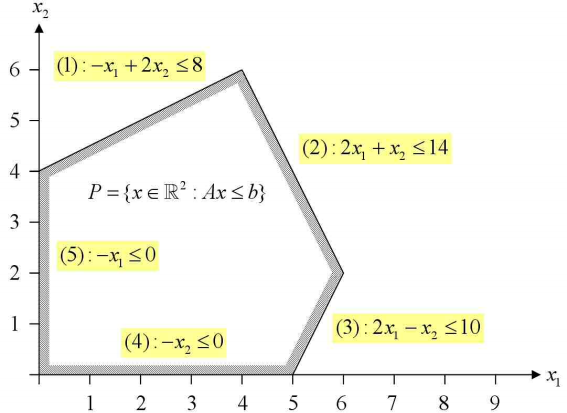
\includegraphics[width=6.3cm]{./Content/LinProg/Hyperplanes}
 	\end{minipage}
 	\begin{minipage}{6.8cm}
 	 	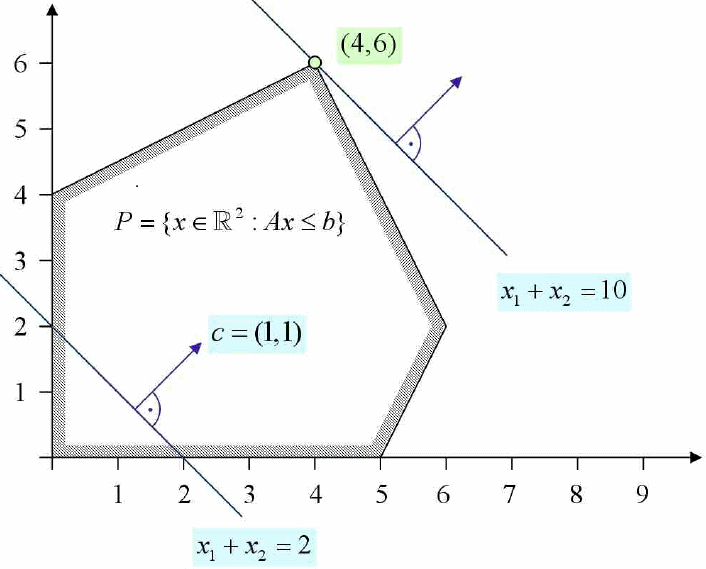
\includegraphics[width=6.3cm]{./Content/LinProg/SolveGraph}
 	\end{minipage}
 	\begin{minipage}{5.9cm}
 	 	 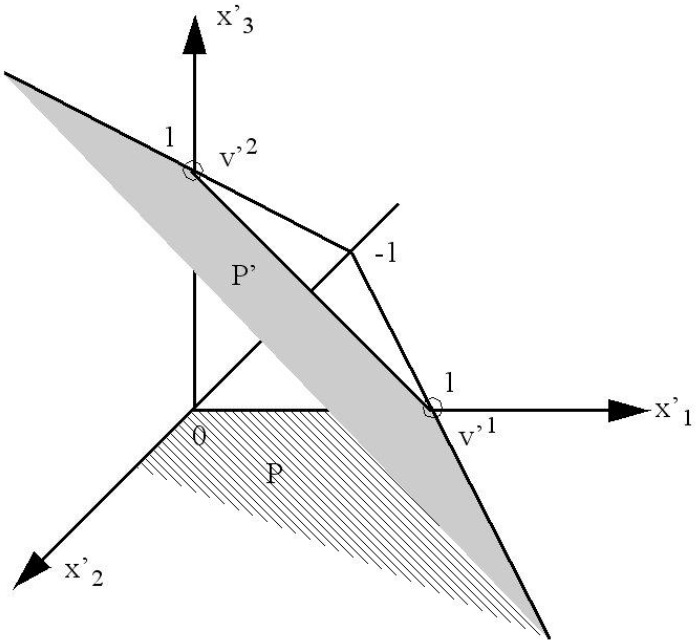
\includegraphics[width=6.3cm]{./Content/LinProg/Koordinatensystem}
 	\end{minipage}
 	
 	  
  \subsubsection{Hyperebenen}
    Die definierenden Hyperebenen sind die Gleichungen, welche den Optimierungsbereich abgrenzen, d.h. pro Gleichung oder Bedingung (in bspw. $Ax \leq b$) entsteht eine Hyperebene. Die Notation lautet z.B. $H_1 = \{x \in \mathbb{R}^3: x_1 + x_2 + x_3 = 2\}$. Die maximale Anzahl von Hyperebenen ist gleich der Anzahl Gleichungen.
    
  \subsubsection{Basisauswahl}
    Es sind bei $n$ Dimensionen $n$ Zeilen auszuwählen. Dabei sollen doppelte Gleichungen von Anfang an ignoriert werden.
    Es sind bis zu $\binom{m}{n}$ Auswahlmöglichkeiten vorhanden ($m$ = \#Gleichungen, $n$ = \#Variablen).
    
    \[ A \in \mathbb{R}^{m\times n} \qquad P = \{ x \in \mathbb{R}^{m\times n} : A x \leq b \} \qquad \qquad \text{Basisauswahl: }B\subseteq \{1,2,...,n\} \qquad  A_B : \text{ Basis von }A \]
    
    \textbf{Bsp.:}
    \[  A=
    	\begin{bmatrix}
    		\textcolor{red}{1} & \textcolor{red}{0} \\
    		1 & 1 \\
    		\textcolor{red}{-1} & \textcolor{red}{1} \\
    		0 & -1
    	\end{bmatrix}
    	\qquad
    	B=\{1,3\} \longrightarrow A_B = 
    	\begin{bmatrix}
 	    		1 & 0 \\
 	    		-1 & 1
    	 \end{bmatrix}
    \]
    
    
  \subsubsection{Basislösung}
  	Berechnung der Basislösung von $P = \{ x \in \mathbb{R}^{m\times n} : A x \leq b \}$ und $B\subseteq \{1,2,...,n\}$:
  	\[ x = A_B^{-1} \cdot b_B \]
  	Die \textbf{Basislösung} ist \textbf{gültig} wenn $\mathbf{x \in P}$ und entspricht dann einem Eckpunkt $v=x$ des Polyeders $P$!!!!
    Um die Basislösung zu bestimmen muss $\mathbf{\det(A_B)\neq 0}$ sein (linear unabhängig).
    
%    Aus Übung 3-2e: $B_1 = \{1,3,5\}:$\\
%    $x_{B_1} = \begin{bmatrix}
%      1 & 1 & 1\\
%      0 & 1 & 0\\
%      -1 & 0 & 0\\
%    \end{bmatrix}^{-1} \begin{bmatrix}
%      2\\ 1 \\0
%    \end{bmatrix} \underbrace{=}_{\text{Zeilen müssen linear unabhängig sein!}} \begin{bmatrix}
%      0\\ 1 \\ 1
%    \end{bmatrix} \underbrace{=}_{\text{Wenn Eckpunkt, dann ist Basisauswahl zulässig}} v_k$
    
%\subsection{Simplex Algorithmus \skript{56}}
%  Siehe auch Übungen 4, Aufgabe 3.
%  
%  \begin{aufzaehlung}
%    \item Als Maximierungsproblem mit $\leq$ Bedingungen umformulieren
%    \item In Matrixschreibweise umschreiben (Matrix $A$ mit einer Variable pro Spalte und einer 
%      Bedingung pro Zeile, $b$ als Spaltenvektor mit einer Bedingung pro Zeile, $c$ als 
%      Zeilenvektor mit den Koeffizienten der Maximierung)
%    \item Basisauswahl $B$ (Menge) bestimmen indem an jeweiligem Eckpunkt $v$ (Spaltenvektor) die betroffenen Bedingungen
%          festgestellt werden.
%    \item Iterationen mit jeweiligem Eckpunkt (Bsp. Bild von $v=(2,4)^T$):
%        
%        \begin{center}
%        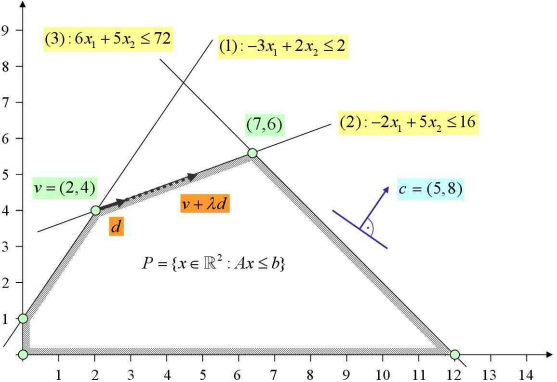
\includegraphics[width=9cm]{./Content/LinProg/simplex}
%        \end{center}
%  
%        \begin{aufzaehlung}
%          \item Basisinverse $\bar{A} = A_B^{-1}$ und evtl. zur Kontrolle Basislösung (= Eckpunkt) $v = \bar{A} b_B$ berechnen
%          \item Reduzierte Kosten berechnen: $u = c \bar{A}$
%          \item Wenn $u \geq 0$, dann Stopp!
%          \item ($u \ngeq 0$). Wähle Spalte $j \in B$ in $u$ ($u_j < 0$) und berechne daraus 
%            $d = - \bar{A}_j$, wobei $j$ in $\bar{A}_j$ die Spalte indiziert. $d$ entspricht der 
%            Richtung, in der vom Eckpunkt weitergesucht wird.
%          \item Stelle die Ungleichung $A v + \lambda A d \leq b$ mit $\lambda \in \mathbb{R}_0$ auf.
%          \item Wenn $Ad \leq 0$, dann ist die grösste Zahl $\lambda$ welche obige Ungleichung erfüllt
%            $\lambda^* = \infty$ und es muss gestoppt werden.
%          \item ($0 \leq \lambda^* < \infty$). Berechne 
%            $\lambda^* = \min \left\{ \frac{b_k - (Av)_k}{(Ad)_k} : k \in \{1,\ldots,m\}, (Ad)_k > 0 \right\}$,
%            d.h. beachte nur Zeilen, wo $(Ad)_k > 0$ ist und berechne den Bruch; der kleinste Index $k$ 
%            ist gesucht.
%          \item Bilde neue zulässige Basisauswahl $B' = B - \{j\} \cup \{k\}$, wobei $j$ in die 
%            Indizierung von der Basismatrix $A_B$ in der ursprünglichen $A$-Matrix zurückberechnet
%            werden soll.
%          \item Neuer Eckpunkt: $v' = v + \lambda^* d$
%          \item Nächste Iteration mit $B = B'$ und $v = v'$ \ldots
%        \end{aufzaehlung}
%      \item Die Optimallösung: $f(v) = cv$
%  \end{aufzaehlung}
%  
%\todo{Beispiel mit Zahlen!!!!!}

\
